As a first step in the evaluation of our grammar-guided evolutionary search method, we consider two PDE-based model problems, Poisson's equation and a linear elastic boundary value problem, which can already be solved efficiently through iterative application of common multigrid cycles .
Here, our goal is, first of all, to demonstrate that our approach is able to reliably find functioning multigrid solvers in a number of randomized independent experiments.
Furthermore, since the known multigrid cycles already provide a strong baseline for these problems, we can investigate whether the methods evolved by our approach are able to achieve a similarly high degree of efficiency.
In addition, by considering both two and three-dimensional problems as well as a system of PDEs, we can demonstrate that our implementation is able to handle PDEs of different type.
\section{Evolving Monolithic Multigrid Solvers}
As it has been mentioned above, the goal of this section is to evaluate the effectiveness of our evolutionary search method in evolving multigrid methods that can be used as a standalone method for the numerical solution of a given PDE.
Therefore, the problem instances considered in this section are chosen in a way that facilitates their efficient solution by multigrid.
This is reflected in the fact that common multigrid cycles, as described in Section~\ref{sec:multigrid-cycles}, are able to quickly converge to the correct solution of each of the resulting systems of linear equations.
We begin this section by introducing the considered problem instances and their mathematical formulation.
At this point we want to emphasize that all results presented in this section have been originally published as part of the paper~\cite{schmitt2021evostencils}.
However, this thesis complements this work with an additional analysis of the multigrid solvers obtained with out evolutionary search method.
\subsection{Poisson's Equation}
\label{sec:poisson-equation}
Poisson's equation is an elliptic PDE that occurs in the study of many physical phenomena~\cite{folland2020introduction} and is defined as
\begin{equation}
	\begin{split}
		-\nabla^{2} u & = f \quad \text{in} \; \Omega \\
		u & = g \quad \text{on} \; \partial \Omega.
	\end{split}
	\label{eq:poisson}
\end{equation}
In our experimental evaluation, we consider two different instances of Poisson's equation with Dirichlet boundary conditions, which are summarized in Table~\ref{table:poisson-problems}.
\begin{table}
	\begin{tabular}{r l l}
		\toprule
		Problem & 2D Poisson & 3D Poisson \\
		\midrule
		$\Omega = $ & $ (0, 1)^2$ & $(0, 1)^3$ \\
		\midrule
		$f(\bm{x}) = $ & $\pi^2 \cos(\pi x) - 4 \pi^2 \sin(2 \pi y)$ & $x^2 - 0.5 y^2 - 0.5 z^2$ \\
		\midrule
		$g(\bm{x}) = $ & $\cos(\pi x) - \sin(\pi y)$ & $0$ \\
		\bottomrule
	\end{tabular}
	\caption{Poisson problem instances.}
	\label{table:poisson-problems}
\end{table}
Note that in Section~\ref{sec:execution-time-analysis} we have utilized the same two-dimensional instance of Poisson's equation to estimate the relative cost of each operation within our evolutionary search method.
We discretize the Laplace operator $\nabla^{2}$ with finite differences on a uniform cartesian grid with step size $h = 1/2^{l_{max}}$.
As a consequence, we obtain the five point stencil
\begin{equation*}
	\nabla^2_h = 
	\frac{1}{h^2} \begin{bmatrix}
		0 & 1 & 0\\
		1 & -4 & 1 \\
		0 & 1 & 0  
	\end{bmatrix},
\end{equation*}
in two dimensions and the seven point stencil
\begin{equation*}
\nabla^2_h = 
\frac{1}{h^2} \begin{bmatrix}
	\begin{bmatrix}
	0 & 0 & 0 \\
	0 & 1 & 0 \\
	0 & 0 & 0
	\end{bmatrix}
	&		
	\begin{bmatrix}
	0 & 1 & 0 \\
	1 & -6 & 1 \\
	0 & 1 & 0 
	\end{bmatrix} &
	\begin{bmatrix}
	0 & 0 & 0 \\
	0 & 1 & 0 \\
	0 & 0 & 0
\end{bmatrix}
\end{bmatrix}
\end{equation*} in three dimensions.
We choose a maximum level of $l_{max} = 11$ in 2D and $l_{max} = 7$ in 3D, which yields systems of linear equations consisting of $4\,190\,209$ and $2\,048\,383$ unknowns, respectively.

\subsection{Linear Elasticity}
Linear elasticity is a fundamental branch of solid mechanics with numerous applications in engineering and material science~\cite{holzapfel2001nonlinear}.
It is derived from the more general theory of nonlinear continuum mechanics by assuming a linear relationship between stress and strain during elastic deformation.
We consider a two-dimensional linear elastic boundary value problem given by the system of PDEs
\begin{equation}
	\begin{split}
		(\alpha + \beta) \cdot (\frac{\partial^2}{\partial x^2} u + \frac{\partial^2}{\partial x \partial y} v) + \alpha \nabla^2 u & = 0 \quad \text{in} \; \Omega \\
		(\alpha + \beta) \cdot (\frac{\partial^2}{\partial x \partial y} u + \frac{\partial^2}{\partial y^2} v) + \alpha \nabla^2 v & = 0 \quad \text{in} \; \Omega \\
		u = 0 \quad \text{and} \quad v & = g \quad \text{on} \; \partial \Omega 
		\label{eq:linear-elasticity}
	\end{split}
\end{equation}
where $\Omega = (0,1)^2$, $\alpha = 195$, $\beta = 130$ and
\begin{equation*}
	g(x,y) = 0.4 \, (1 - x) \, x y \, \sin(\pi x).
\end{equation*}
From a physical point of view, this system can be interpreted as a two-dimensional rectangular body that undergoes an elastic deformation into y-direction, as it can be seen in Figure~\ref{fig:visualization-linear-elasticity}.
\begin{figure}
	\centering
	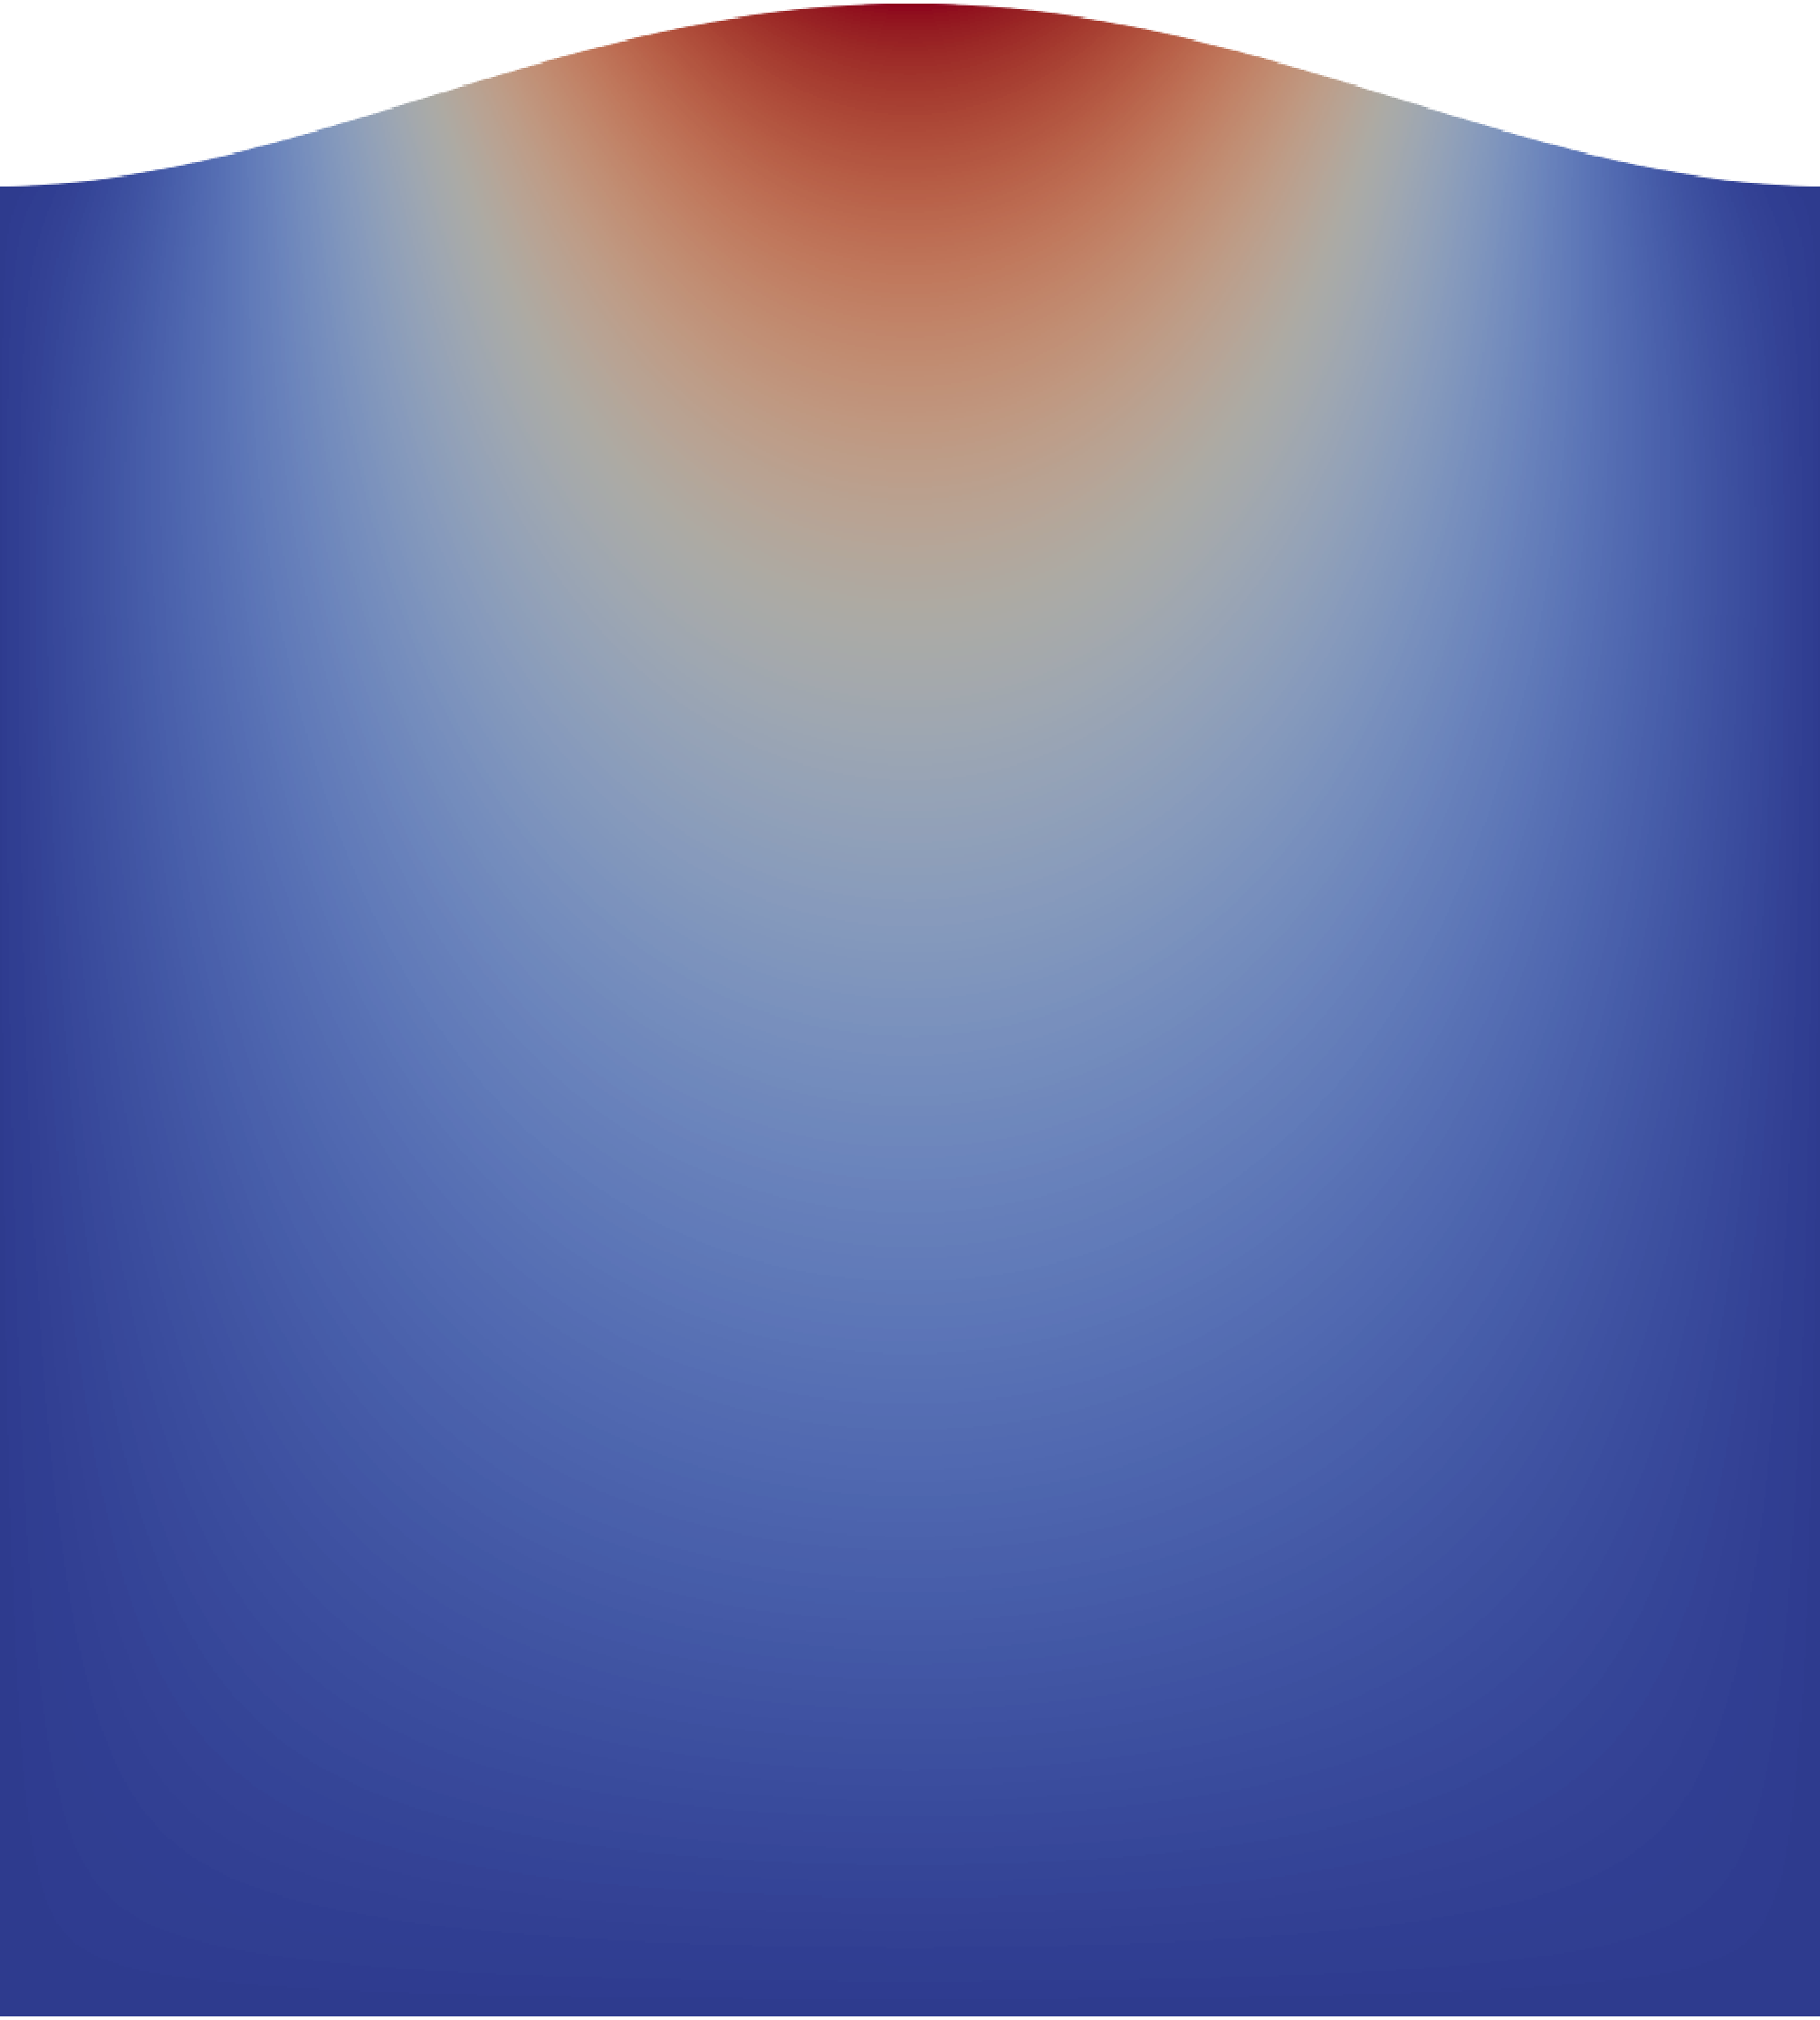
\includegraphics[width=0.5\textwidth]{figures/visualization-linear-elasticity1}
	\caption{Visualization of the considered linear elastic boundary value problem. A two-dimensional rectangular body undergoes an elastic deformation into y-direction.}
	\label{fig:visualization-linear-elasticity}
\end{figure}
We discretize equation \eqref{eq:linear-elasticity} with finite differences on a cartesian grid using a step size $h = 1/2^{l_{max}}$ with $l_{max} = 10$, which yields a system of linear equations $\boldsymbol{A} \boldsymbol{u} = \boldsymbol{f}$ with 
\begin{equation*}
	\boldsymbol{A} =
	\begin{pmatrix}
		(\alpha + \beta) \frac{\partial^2}{\partial x^2} + \alpha \nabla^2 & (\alpha + \beta) \frac{\partial^2}{\partial x \partial y} \\
		(\alpha + \beta) \frac{\partial^2}{\partial x \partial y} & (\alpha + \beta) \frac{\partial^2}{\partial y^2} +  \alpha \nabla^2
	\end{pmatrix},
\end{equation*}
\begin{equation*}
	\boldsymbol{u} = \begin{pmatrix}
		u \\ v
	\end{pmatrix}, \quad
	\boldsymbol{f} =
	\begin{pmatrix}
		f_{u} \\ f_{v}
	\end{pmatrix} =
	\begin{pmatrix}
		0 \\ 0
	\end{pmatrix},
\end{equation*}
whereby the differential operators $\nabla^2$, $\frac{\partial^2}{\partial x^2}$, $\frac{\partial^2}{\partial y^2}$ and $\frac{\partial^2}{\partial x \partial y}$ are approximated by their discrete counterparts
\begin{equation*}
	\left(\nabla^2 u\right)_{i,j} = 
	\frac{1}{h^2} \begin{bmatrix}
		0 & 1 & 0\\
		1 & -4 & 1 \\
		0 & 1 & 0  
	\end{bmatrix},
\end{equation*}
\begin{equation*}
	\left(\frac{\partial^2}{\partial x^2} u\right)_{i,j} =
		\frac{1}{h^2} \begin{bmatrix}
		0 & 0 & 0\\
		1 & -2 & 1 \\
		0 & 0 & 0  
	\end{bmatrix},
\end{equation*}
\begin{equation*}
	\left(\frac{\partial^2}{\partial y^2} u\right)_{i,j} =
	\frac{1}{h^2} \begin{bmatrix}
		0 & 1 & 0\\
		0 & -2 & 0 \\
		0 & 1 & 0  
	\end{bmatrix},
\end{equation*}
\begin{equation*}
	\left(\frac{\partial^2}{\partial x \partial y} u\right)_{i,j} = 
	\frac{1}{4 h^2} \begin{bmatrix}
		-1 & 0 & 1\\
		0 & 0 & 0 \\
		1 & 0 & -1  
	\end{bmatrix}.
\end{equation*}
Similar to the above case, we employ a uniform cartesian grid of size $h = 1/l_{max}$ with $l_{max} = 10$, such that the resulting system of linear equations contains $2\,093\,058$ unknowns.
\subsection{Multigrid Configuration}
To design a multigrid method, we consider each of the given problems a grid hierarchy consisting of five discretization levels $l \in \left[l_{max} - 4, l_{max}\right]$, where the grid spacing on each level is given by the formula $h = 1/2^l$.
We then obtain the respective operator on each level by applying the same discretization method as described above.
Therefore, the resulting grammar is structurally similar to the one shown in Table~\ref{table:multigrid-grammar}.
Within each grammar production rule, we then consider the following components:
\begin{description}
	\item[\textbf{Smoothers}:] Decoupled / Collective Jacobi and red-black Gauss-Seidel, block Jacobi with rectangular blocks up to a maximum number of 6 terms.
	\item[\textbf{Restriction}:] Full-weighting restriction.
	\item[\textbf{Prolongation}:] Bilinear interpolation.
	\item[\textbf{Relaxation factors}:] $\omega \in \left( 0.1 + 0.05i \right)_{i = 0}^{36} = \left(0.1, 0.15, 0.2, \dots 1.9 \right)$
	\item[\textbf{Coarse-grid solver}:] Conjugate gradient method for $l = l_{max} - 4$.
\end{description}
Here, we generate block Jacobi smoothers by defining a splitting $A = L + D + U$ where $D$ is a block diagonal matrix of the form
\begin{equation*}
	D = 
		\begin{pmatrix}A_{11}&0&\cdots &0\\
			0&A_{22}&\cdots &0\\
			\vdots &\vdots &\ddots &\vdots \\0&0&\cdots &A_{mm}\end{pmatrix},
\end{equation*}
where each matrix $A_{ij}$ corresponds to a set of adjacent grid points contained in the respective rectangular block, as it has been discussed in Section~\ref{subsec:block-smoothing}.
A more detailed treatment of block relaxation methods can be found in~\cite{trottenberg2000multigrid}.
For each of smoothing and coarse-grid correction step the relaxation factor $\omega$ is chosen from the above sequence.
As a baseline for assessing the efficiency and generalizability of the evolved multigrid solvers, we consider a number of common multigrid cycles with red-black Gauss-Seidel smoothing and optimized relaxation factors.
We, therefore, formulate these methods on the same five-grid hierarchy, whereby we also utilize the same restriction, prolongation operators and coarse-grid solver, as described above.
In each case, we consider the corresponding linear system as solved when the initial residual has been reduced by a factor of $10^{-12}$.
\subsection{Optimization Settings and Evaluation Platform}
\label{sec:optimization-settings}
After specifying the operator and parameter choices considered within the construction of each multigrid solver, we next describe the settings under which we perform each GP-based optimization run.
Here, we utilize the EvoStencils framework, whose implementation has been described in detail in Chapter~\ref{chapter:evostencils-1} and~\ref{chapter:evostencils-2}.
The goal of each optimization run is then to evolve the set of non-dominated according to the two objectives convergence factor $\rho$ and execution time per iteration $t$, as described in Section~\ref{sec:fitness-evaluation-and-selection}, which are evaluated by applying each multigrid method as an iterative solver to the respective test problem.
The resulting individuals are then subject to a subsequent evaluation and comparison with the available reference methods. 
Table~\ref{table:gp-parameters} gives an overview about the configuration of the EvoStencils framework used within each experiment.
\begin{table}
	\centering
	\caption{Summary of GGGP configuration parameters.}
	\label{table:gp-parameters}
	\begin{tabular}{l c}
		\toprule
		Parameter & Value \\
		\midrule 
		Evolutionary algorithm type & $(\mu + \lambda)$ \\
		\midrule
		Objectives & $t, \rho$ \\
		\midrule
		Number of generations & 250 \\
		\midrule
		Initial population size & 2048 \\
		\midrule
		$\lambda$ & 256 \\
		\midrule
		$\mu$ & 256 \\
		\midrule
		Number of MPI processes & 64 \\
		\midrule
		Non-dominated sorting procedure & \cite{deb2002fast} \\ 
		\midrule
		Selection operator & \cite{deb2002fast} \\ 
		\midrule
		Crossover operator & Single-point crossover \\
		\midrule
		Crossover probability & $2/3$ \\
		\midrule
		Mutation operator & Random subtree replacement \\
		\midrule 
		Probability to mutate a terminal symbol & $1/3$ \\
		\bottomrule
	\end{tabular}
\end{table}
Within each run, starting with a randomly generated population of 2048 individuals, we perform an evolutionary search for 250 generations.
In each generation, we create new individuals by first selecting $\lambda = 256$ candidates from the current population.
We then apply mutation and crossover to each pair of selected candidates to create two child individuals, whereby the crossover probability is set to $2/3$ and in case of mutation we choose terminal symbol with a probability of $1/3$.
The resulting individuals are then evaluated according to the two objectives by generating a parallel C++ solver implementation using the ExaStencils framework, which is then applied to the respective problem as described above.
Hereby we distribute the evaluation of all 256 individuals to 64 MPI processes, such that each process is responsible for the evaluation of exactly four individuals.
The resulting fitness values are then distributed to all 64 processes, such that each of them possesses an identical copy of each child individual together with its fitness value, as it has been described in Chapter~\ref{sec:distributed-parallelization}.
Finally, we select $\mu = 256$ individuals as a population for the next generation from the combined set of parent and child individuals using the NSGA-II non-dominated sorting procedure~\cite{deb2002fast}.

As an evaluation platform for running each experiment, we employ 32 nodes of the Meggie compute cluster of the Erlangen National High Performance Computing Center (NHR), where each node of the system consists of two sockets, each with ten physical CPU cores.
Therefore, each process is pinned and executed on a dedicated socket, while for the evaluation of each solver we employ a thread-based parallelization using ten OpenMP threads, where each tread is pinned to a distinct physical compute core on the respective socket.
For the parallelization of each nested loop, we employ a static scheduling based on the outer loop, such that each threads processes a consecutive chunk of iterations.
To generate a thread-parallel executable for each solver, we employ GCC 9.3.0 with the -O3 optimization level.
Finally, we execute each solver three times and then compute the average for both objectives to reduce statistical variations between individual evaluation runs.

\subsection{Algorithm Behavior Analysis}
As a first step towards a quantitative evaluation of our evolutionary search method, we assess whether our algorithm is able to effectively find good solutions with respect to our two optimization objectives.
For this purpose, we measure the minimum of each of the two objectives within the population throughout each of the ten optimization runs for all three test problems.
As a result, Figure~\ref{fig:poisson-2D-minimum-objectives},~\ref{fig:poisson-3D-minimum-objectives} and~\ref{fig:linear-elasticity-2D-minimum-objectives} shows the mean and standard deviation of the current optimum of both objectives over each of the ten optimization runs.
\begin{figure}
	\centering
	\begin{subfigure}[b]{0.49\textwidth}
		\centering
		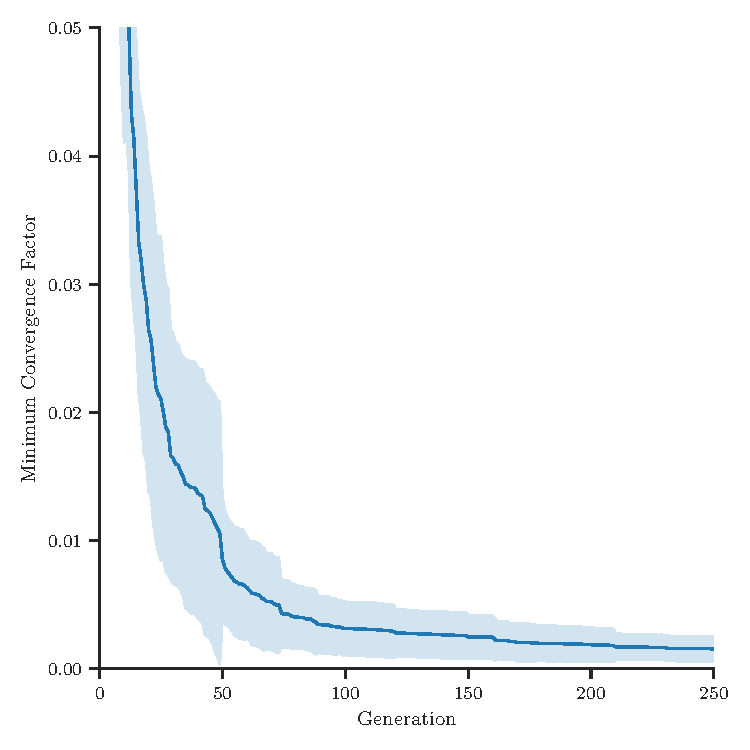
\includegraphics[width=\textwidth]{figures/minimum_convergence_factor_2D_FD_Poisson_fromL2.pdf}
		\caption{Minimum Convergence Factor}
		\label{fig:poisson-2D-minimum-convergence-factor}
	\end{subfigure}
	\hfill
	\begin{subfigure}[b]{0.49\textwidth}
		\centering
		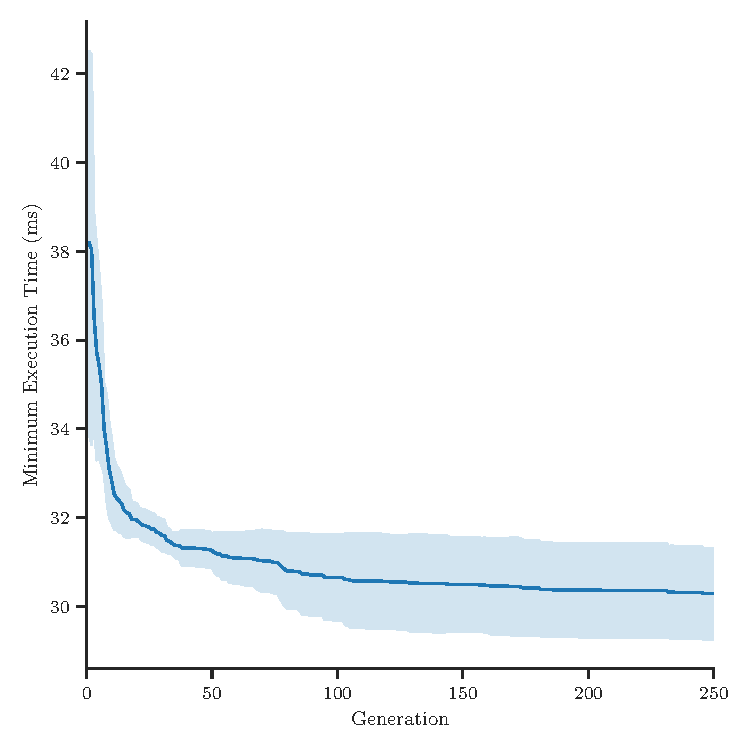
\includegraphics[width=\textwidth]{figures/minimum_execution_time_2D_FD_Poisson_fromL2.pdf}
		\caption{Minimum Execution Time per Iteration}
		\label{fig:poisson-2D-minimum-execution-time}
	\end{subfigure}
	\caption{2D Poisson - Mean and standard deviation of the minimum objective function values during the optimization.}
	\label{fig:poisson-2D-minimum-objectives}
\end{figure}
\begin{figure}
	\centering
	\begin{subfigure}[b]{0.49\textwidth}
		\centering
		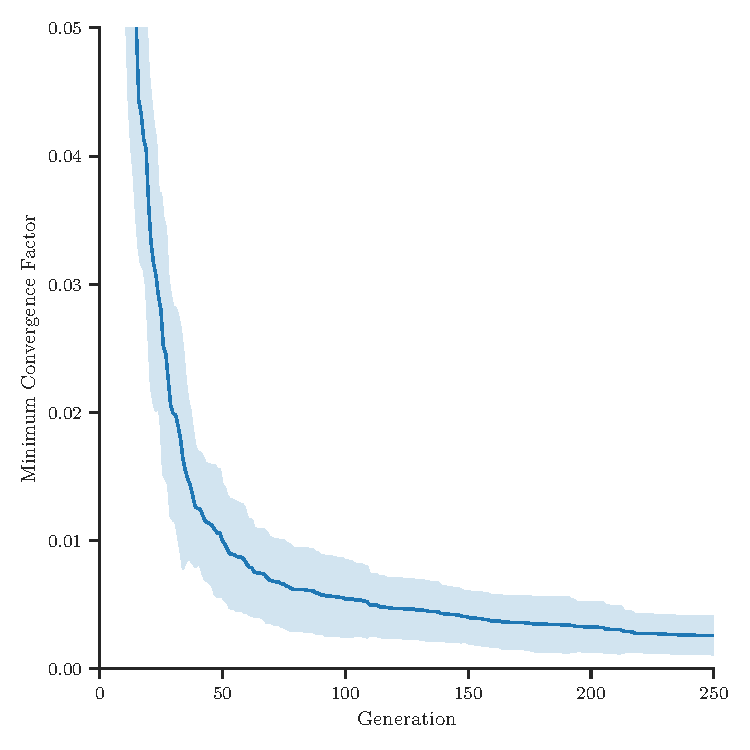
\includegraphics[width=\textwidth]{figures/minimum_convergence_factor_3D_FD_Poisson_fromL2.pdf}
		\caption{Minimum Convergence Factor}
		\label{fig:poisson-3D-minimum-convergence-factor}
	\end{subfigure}
	\hfill
	\begin{subfigure}[b]{0.49\textwidth}
		\centering
		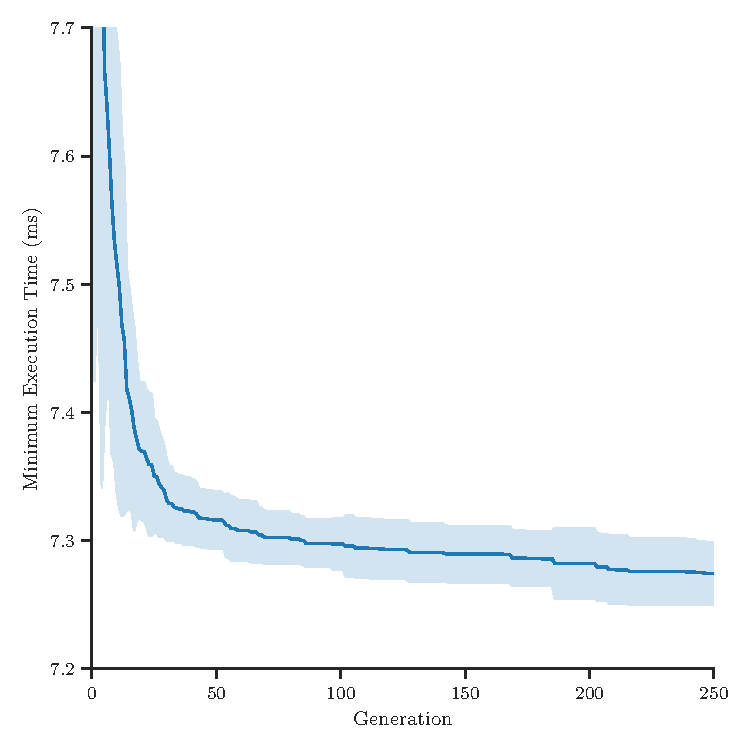
\includegraphics[width=\textwidth]{figures/minimum_execution_time_3D_FD_Poisson_fromL2.pdf}
		\caption{Minimum Execution Time per Iteration}
		\label{fig:poisson-3D-minimum-execution-time}
	\end{subfigure}
	\caption{3D Poisson - Mean and standard deviation of the minimum objective function values during the optimization.}
	\label{fig:poisson-3D-minimum-objectives}
\end{figure}
\begin{figure}
	\centering
	\begin{subfigure}[b]{0.49\textwidth}
		\centering
		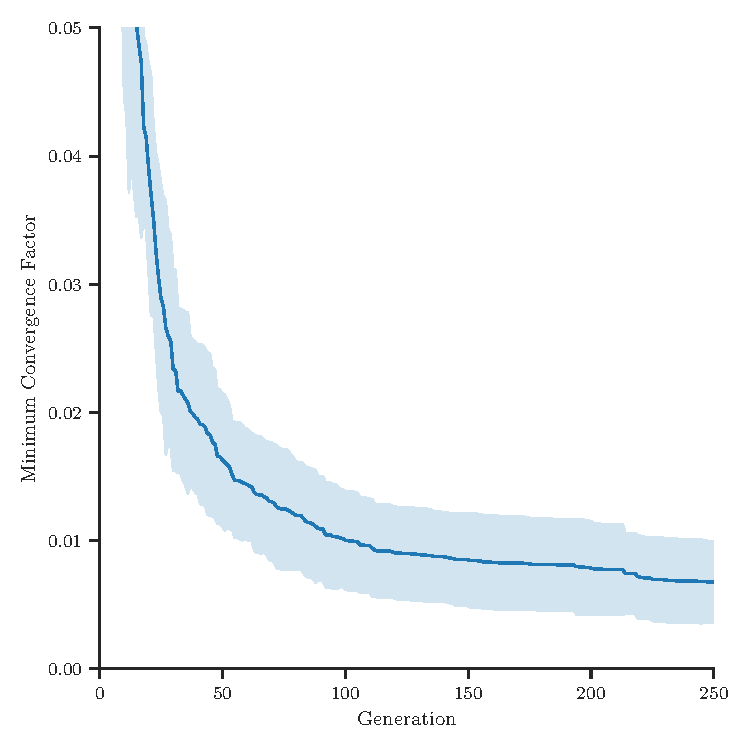
\includegraphics[width=\textwidth]{figures/minimum_convergence_factor_2D_FD_LinearElasticity_fromL2.pdf}
		\caption{Minimum Convergence Factor}
		\label{fig:linear-elasticity-2D-minimum-convergence-factor}
	\end{subfigure}
	\hfill
	\begin{subfigure}[b]{0.49\textwidth}
		\centering
		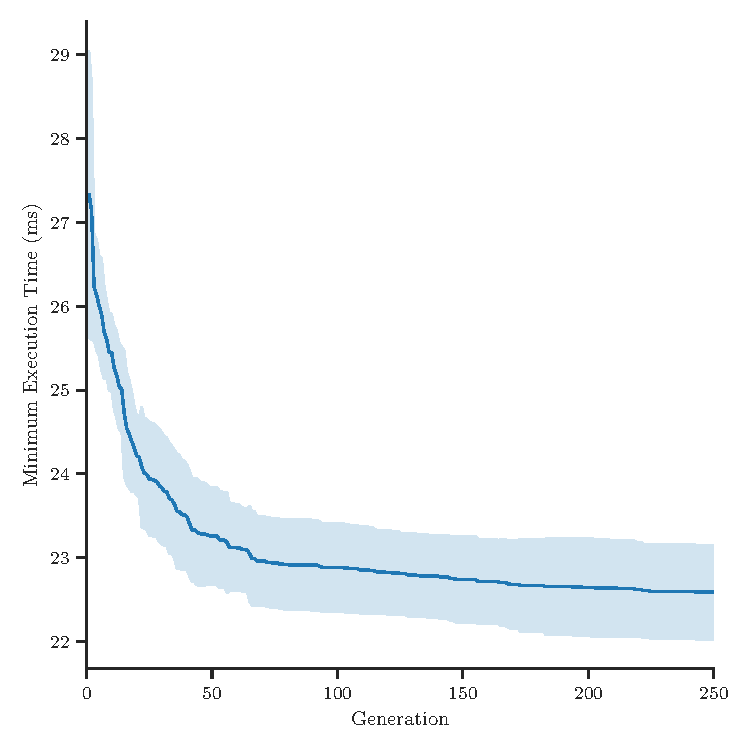
\includegraphics[width=\textwidth]{figures/minimum_execution_time_2D_FD_LinearElasticity_fromL2.pdf}
		\caption{Minimum Execution Time per Iteration}
		\label{fig:linear-elasticity-2D-minimum-execution-time}
	\end{subfigure}
	\caption{2D Linear Elasticity - Mean and standard deviation of the minimum objective function values during the optimization.}
	\label{fig:linear-elasticity-2D-minimum-objectives}
\end{figure}
First of all, in general we can assess that in all three cases our algorithm is able to quickly reduce the minimum value of both objectives within the population.
However, if we compare the slope of the two objectives for the three different problems, we can see that in case of the first objective $\rho$ significantly more generations are required to achieve the same degree of reduction as for the second objective $t$.
In all three cases, the algorithm still significantly improves upon the current minimum of $\rho$ beyond the first 50 generations, which can be seen in Figure~\ref{fig:poisson-2D-minimum-convergence-factor},~\ref{fig:poisson-3D-minimum-convergence-factor} and~\ref{fig:linear-elasticity-2D-minimum-convergence-factor}.
In contrast, for the second objective $t$, the majority of improvement happens within the first 50--70 generations, as it can be seen in Figure~\ref{fig:poisson-2D-minimum-execution-time},~\ref{fig:poisson-3D-minimum-execution-time} and~\ref{fig:linear-elasticity-2D-minimum-execution-time}.
At this point it is also important to consider that while the convergence factor is constant for each execution of the same solver, $t$ is obtained by measuring its execution time on the respective compute node.
Therefore, due to manufacturing and temperature-based variations, we can expect a certain degree of fluctuations when measuring the execution time of the same solver on different compute nodes during consecutive optimization runs.
Consequently, even though the algorithm is more effective in quickly reducing the second objective, this results in a larger deviations between individual optimizations runs and, thus, a overall higher standard deviation.

Second, by considering the absolute value of the minimum convergence factor attained in each of the three different cases, we can assess the difficulty of the underlying problem.
While the execution time per iteration, as a second objective, is solely determined by the computational complexity of each solver and the properties of the given computer architecture it is executed on, a smaller convergence factor indicates that the underlying problem is easier to solve.
Poisson's equation represents an often-studied model problem, whose strong ellipticity enables its effective solution using multigrid methods~\cite{trottenberg2000multigrid}.
As a consequence, our algorithm is able to consistently evolve multigrid methods that achieve fast convergence, with minimum convergence factors of less than 0.005, in solving both the two and three dimensional instances of this equation, which can be seen in Figure~\ref{fig:poisson-2D-minimum-convergence-factor} and~\ref{fig:poisson-3D-minimum-convergence-factor}.
In case of the linear elastic boundary value problem, both the mean and standard deviation remain higher for the first objective throughout the optimization.
However, on average our algorithm is still able to evolve multigrid methods that achieve a convergence factor of 0.01 of less and, therefore, outstandingly fast convergence.
In summary, we can conclude that our search method is able to consistently find satisfactory minima for both objectives in all three test cases considered.

To further analyze the behavior of our multi-objective evolutionary algorithm, we consider the distribution of non-dominated individuals at the end of all optimization runs, which is shown in Figure~\ref{fig:pareto-front-2D-poisson},~\ref{fig:pareto-front-3D-poisson} and~\ref{fig:pareto-front-2D-linear-elasticity}.
\begin{figure}
	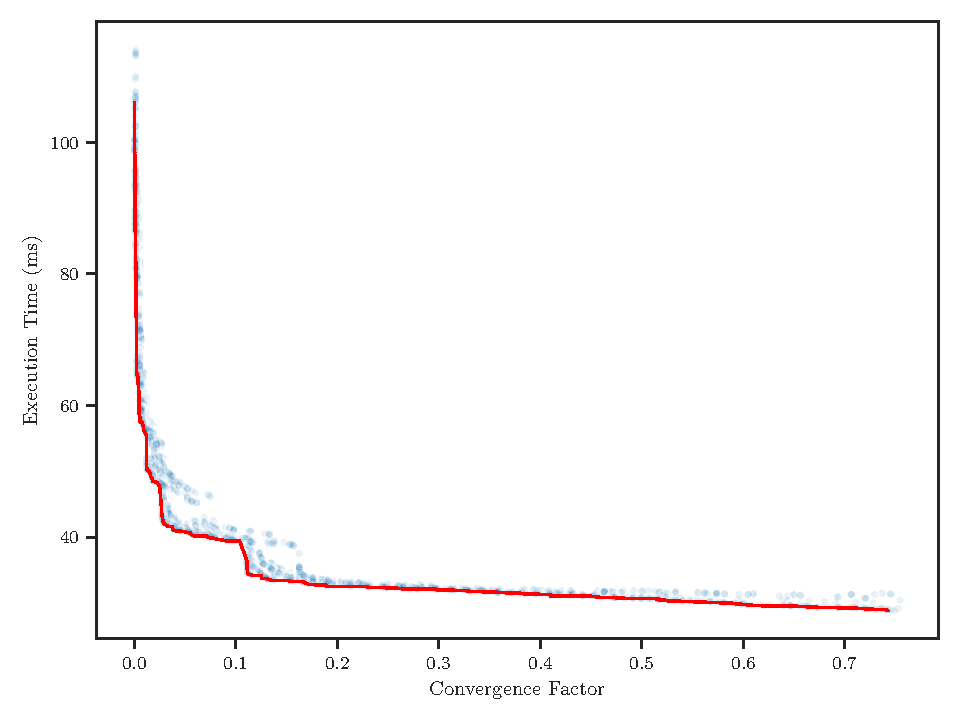
\includegraphics[width=\columnwidth]{figures/pareto_front_2D_FD_Poisson_fromL2.pdf}
	\caption{2D Poisson - Distribution of non-dominated individuals at the end of all ten experiments. The red line denotes the combined Pareto front.}
	\label{fig:pareto-front-2D-poisson}
\end{figure}
\begin{figure}
	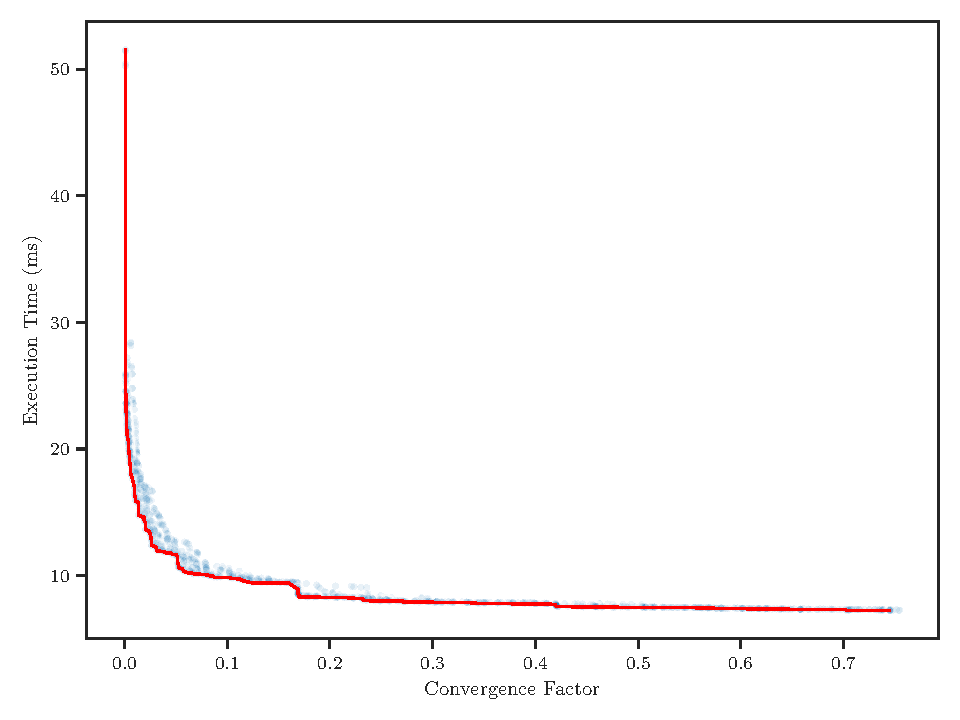
\includegraphics[width=\columnwidth]{figures/pareto_front_3D_FD_Poisson_fromL2.pdf}
	\caption{3D Poisson - Distribution of non-dominated individuals at the end of all ten experiments. The red line denotes the combined Pareto front.}
	\label{fig:pareto-front-3D-poisson}
\end{figure}
\begin{figure}
	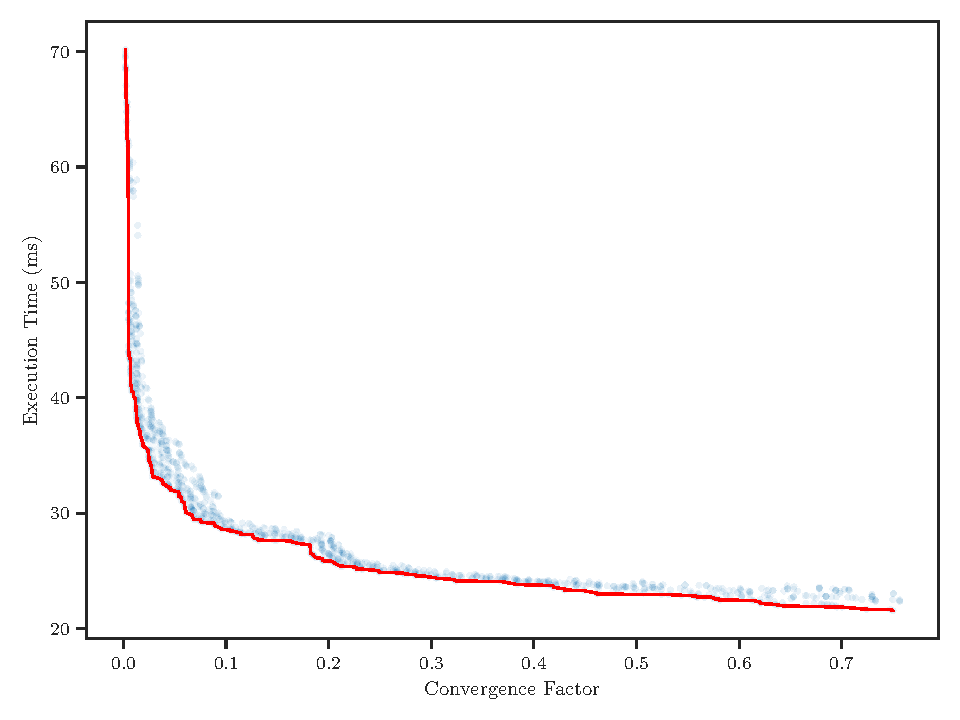
\includegraphics[width=\columnwidth]{figures/pareto_front_2D_FD_LinearElasticity_fromL2.pdf}
	\caption{2D Linear Elasticity - Distribution of non-dominated individuals at the end of all ten experiments. The red line denotes the combined Pareto front.}
	\label{fig:pareto-front-2D-linear-elasticity}
\end{figure}
Here the red line denotes the combined front while the color density of the distribution indicates where the majority of solutions is located at the end of all experiments. 
In all three cases, the majority of non-dominated solutions evolved within each experiment can be found close to the combined front.
While in Figure~\ref{fig:pareto-front-2D-poisson} the number of solutions that are distinctly located outside of the front is slightly higher than in the other two cases, their distance to the next point on this front is still comparably small compared to the complete objective space.
Again we can attribute part of this effect to measurement variations in the solver execution time on different compute nodes.
Furthermore, note that for the most part and especially the center of the objective space, the solutions are evenly distributed alongside the front.
Here only the left-upper part of Figure~\ref{fig:pareto-front-3D-poisson} and~\ref{fig:pareto-front-2D-linear-elasticity} represents a noteworthy exception, where the algorithm struggles to find the same solutions within each run.
This effect can be mainly attributed to the fact that the solutions located at this part of the space are characterized by an extremely fast convergence.
Since the convergence of a multigrid method can be first and foremost accelerated with the addition of smoothing and coarse-grid correction steps, finding the same non-dominated solutions with fast convergence requires us to evolve increasingly large expression of the same structure in individual experiments.
Recently, the limited capabilities of NSGA-II to evolve large non-dominated expressions have been demonstrated in~\cite{liu2022evolvability}, which, therefore, similarly offers an explanation for the impaired evolution of fast-converging solutions in the given case.
\subsection{Comparison with Reference Methods}
Finally, in order to investigate whether our approach yields multigrid methods that are competitive with well-known multigrid cycles, we consider two different recent multi-core CPU architectures for evaluation: Intel Xeon E5-2630v4 (Broadwell) and Intel Xeon 2660v2 (Ivy Bridge).
In both cases, each compute node consists of two sockets with 20 physical CPU cores and a cache-coherent NUMA architecture.
Each solver is then executed on a dedicated node using a thread-based parallelization with 20 OpenMP threads, whereby we pin each thread to a unique physical core and employ the same parallelization approach as described in Section~\ref{sec:optimization-settings}.
In order to assess the solving speed of the methods evolved, we consider two different problem sizes for each of the three test cases.
While in the first case a problem size identical to the one employed within the optimization is chosen, in the second case we obtain a larger one by doubling number of grid points in each dimension.
Even though the evaluation of our methods generalizability is not the focus of this section, it is still worthwhile to investigate whether the methods evolved with our approach also are capable of solving larger instances of the same problem.
For comparison we consider a number of different V-cycles with at most four red-black Gauss-Seidel pre and post-smoothing steps, as these methods are known to lead to the fastest multigrid-based solvers for Poisson's equation according to the classical formulation of multigrid shown in Algorithm~\ref{alg:multigrid-cycle}~\cite{trottenberg2000multigrid}.
As we have already investigated in~\cite{schmitt2020constructing}, the same is true for the linear elastic boundary value problem considered here.
To achieve a fair comparison, we empirically choose the optimum relaxation factor $\omega$ for each test case from the same interval considered within the optimization, which leads to $\omega = 1.15$ for the two-dimensional Poisson equation and $\omega = 1.25$ both for the three-dimensional Poisson equation and the linear elastic boundary value problem.
Table~\ref{table:poisson-2D-reference-methods},~\ref{table:poisson-3D-reference-methods} and~\ref{table:linear-elasticity-2D-reference-methods} contains the resulting solving times and number of iterations to achieve the required defect reduction for the respective test case.
Here, for instance, the abbreviation V(2, 1) denotes a V-cycle with two pre and one post-smoothing step with red-black Gauss-Seidel.
First of all, as we can expect from a functioning multigrid method, the number of iterations stays constant for both problem sizes, only with the exception of the V(1,0)-cycle, where we can observe a slight increase for the linear elastic boundary value problem.
Overall, we can conclude that while the V(2,2)-cycle represents the fastest solver for both cases of Poisson's equation, the V(3,3) cycle leads to the fastest solving time in case of the linear elastic boundary value problem.
\begin{table}
	\caption{2D Poisson - Measured number of iterations and solving times of the reference methods on 20 cores and two sockets.}
	\label{table:poisson-2D-reference-methods}
	\centering
	\begin{tabular}{l c c c c c c}
		\toprule
		& \multicolumn{2}{c}{Iterations} & \multicolumn{2}{c}{Broadwell (ms)} & \multicolumn{2}{c}{Ivy Bridge (ms)} \\
		\cmidrule(r){2-3} \cmidrule(r){4-5} \cmidrule(r){6-7}
		$l_{max}$ & $11$& $12$ & $11$ & $12$ & $11$ & $12$\\
		\midrule
		V(1, 0) & 21 & 21 & 969 & 2810 & 879 & 2652 \\
		\midrule
		V(1, 1) & 9 & 9 & 461 & 1359 & 411 & 1287 \\
		\midrule
		V(2, 1) & 7 & 7 & 377 & 1137 & 334 & 1087\\
		\midrule
		V(2, 2) & 6 & 6 & 344 & 1056 & 302 & 1007 \\
		\midrule
		V(3, 2) & 6 & 6 & 378 & 1160 & 324 & 1112 \\
		\midrule
		V(3, 3) & 6 & 6 & 397 & 1255 & 344 & 1201 \\
		\midrule
		V(4, 3) & 6 & 6 & 425 & 1350 & 366 & 1306 \\
		\midrule
		V(4, 4) & 6 & 6 & 448 & 1449 & 383 & 1409\\
		\bottomrule
	\end{tabular}
	%FMG for max_level = 12: 530.3038500000001 ms, 3 Iterations
\end{table}
\begin{table}
	\caption{3D Poisson - Measured number of iterations and solving times of the reference methods on 20 cores and two sockets.}
	\label{table:poisson-3D-reference-methods}
	\centering
	\begin{tabular}{l c c c c c c}
		\toprule
		& \multicolumn{2}{c}{Iterations} & \multicolumn{2}{c}{Broadwell (ms)} & \multicolumn{2}{c}{Ivy Bridge (ms)} \\
		\cmidrule(r){2-3} \cmidrule(r){4-5} \cmidrule(r){6-7}
		$l_{max}$ & $7$& $8$ & $7$ & $8$ & $7$ & $8$\\
		\midrule
		V(1, 0) & 29 & 30 & 121.3 &1221 & 134.6 & 1470 \\
		\midrule
		V(1, 1) & 13 & 13 & 70.8 & 682 & 79.9 & 838 \\
		\midrule
		V(2, 1) & 9 & 9 & 59.0 & 582 & 66.2 & 708 \\
		\midrule
		V(2, 2) & 7 & 7 & 54.6 & 531 & 65.4 & 654 \\
		\midrule
		V(3, 2) & 7 & 7 & 61.9 & 610 & 74.6 & 757 \\
		\midrule
		V(3, 3) & 7 & 7 & 72.6 & 690 & 86.6 & 857 \\
		\midrule
		V(4, 3) & 7 & 6 & 77.9 & 656 & 87.3 & 825 \\
		\midrule
		V(4, 4) & 6 & 6 & 73.2 & 725 & 82.5 & 906 \\
		\bottomrule
	\end{tabular}
\end{table}
\begin{table}
	\caption{2D Linear Elasticity - Measured number of iterations and solving times of the reference methods on 20 cores and two sockets.}
	\label{table:linear-elasticity-2D-reference-methods}
	\centering
	\begin{tabular}{l c c c c c c}
		\toprule
		& \multicolumn{2}{c}{Iterations} & \multicolumn{2}{c}{Broadwell (ms)} & \multicolumn{2}{c}{Ivy Bridge (ms)} \\
		\cmidrule(r){2-3} \cmidrule(r){4-5} \cmidrule(r){6-7}
		$l_{max}$ & $10$& $11$ & $10$ & $11$ & $10$ & $11$\\
		\midrule
		V(1, 0) & 32 & 31 & 872 & 4306 & 828 & 4128 \\
		\midrule
		V(1, 1) & 15 & 15 & 439 & 2118 & 418 & 2075\\
		\midrule
		V(2, 1) & 10 & 10 & 318 & 1529 & 312 & 1529 \\
		\midrule
		V(2, 2) & 9 & 9 & 314 & 1449 & 316 & 1476 \\
		\midrule
		V(3, 2) & 8 & 8 & 297 & 1368 & 304 & 1388 \\
		\midrule
		V(3, 3) & 7 & 7 & 283 & 1247 & 288 & 1288 \\
		\midrule
		V(4, 3) & 7 & 7 & 293 & 1320 & 313 & 1397 \\
		\midrule
		V(4, 4) & 7 & 7 & 311 & 1378 & 334 & 1471 \\
		\bottomrule
	\end{tabular}
\end{table}

Finally, we can then evaluate the multigrid methods obtained with our grammar-guided search method in each of the ten experiments under the same conditions.
As the number of non-dominated individuals within the population at the end of each run is unrestricted and can, therefore, be too high for a direct evaluation, we heuristically identify the 50 most promising individuals by sorting them according to the metric
\begin{equation}
	T_{\varepsilon} = \frac{\log(\varepsilon)}{\log(\rho)} \cdot t,
\end{equation}
where $\varepsilon = 10^{-12}$ is the desired defect reduction factor and $\rho$ and $t$ the objective function values obtained within the optimization.
Each of the resulting methods is then executed as a solver for the respective test problem on a Broadwell compute node consisting of two sockets with 20 CPU cores, whereby we employ the same problem size as within the optimization.
Note that while the problem size and computer architecture is identical to the one used within the optimization, increasing the number of CPU cores leads to a higher degree of parallelism and, thus, smaller execution time per iteration, which necessitates the reevaluation of each method.
After we have identified the method that leads to the fastest solver in each experiment, we execute it on both problem sizes and evaluation platforms, as described above.
Table~\ref{table:poisson-2D-evolved-methods},~\ref{table:poisson-3D-evolved-methods} and~\ref{table:linear-elasticity-2D-evolved-methods} contain the resulting measured solving times for each case.
\begin{table}
	\caption{2D Poisson - Measured number of iterations and solving times of the evolved multigrid methods on 20 cores and two sockets.}
	\label{table:poisson-2D-evolved-methods}
	\centering
	\begin{tabular}{l c c c c c c}
		\toprule
		& \multicolumn{2}{c}{Iterations} & \multicolumn{2}{c}{Broadwell (ms)} & \multicolumn{2}{c}{Ivy Bridge (ms)} \\
		\cmidrule(r){2-3} \cmidrule(r){4-5} \cmidrule(r){6-7}
		$l_{max}$ & $11$& $12$ & $11$ & $12$ & $11$ & $12$\\
		\midrule
		ES-1 & 5 & 5 & 338 & 1064 & 304 & 1055\\
		\midrule
		ES-2 & 6 & 6 & 371 & 1163 & 330 & 1133 \\
		\midrule
		ES-3 & 5 & 5 & 311 & 988 & 279 & 976 \\
		\midrule
		ES-4 & 6 & 6 & 380 & 1188 & 338 & 1153 \\
		\midrule
		ES-5 & 5 & 5 & 312 & 978 & 279 & 963 \\
		\midrule
		ES-6 & 5 & 5 & 349 & 1123 & 309 & 1106 \\
		\midrule
		ES-7 & 6 & 6 & 354 & 1096 & 320 & 1068 \\
		\midrule
		ES-8 & 6 & 6 & 347 & 1081 & 310 & 1056 \\
		\midrule
		ES-9 & 6 & 6 & 353 & 1079 & 313 & 1045 \\
		\midrule
		ES-10 & 5 & 5 & 310 & 960 & 275 & 934 \\
		\bottomrule
	\end{tabular}
\end{table}
\begin{table}
	\caption{3D Poisson - Measured number of iterations and solving times of the evolved multigrid methods on 20 cores and two sockets.}
	\label{table:poisson-3D-evolved-methods}
	\centering
	\begin{tabular}{l c c c c c c}
		\toprule
		& \multicolumn{2}{c}{Iterations} & \multicolumn{2}{c}{Broadwell (ms)} & \multicolumn{2}{c}{Ivy Bridge (ms)} \\
		\cmidrule(r){2-3} \cmidrule(r){4-5} \cmidrule(r){6-7}
		$l_{max}$ & $7$& $8$ & $7$ & $8$ & $7$ & $8$\\
		\midrule
		ES-1 & 10 & 11 & 55.3 & 577 & 70.0 & 704\\
		\midrule
		ES-2 & 8 & 9 & 57.2 & 578 & 64.3 & 716 \\
		\midrule
		ES-3 & 8 & 9 & 59.0 & 671 & 65.3 & 824 \\
		\midrule
		ES-4 & 8 & 9 & 54.6 & 576 & 62.7 & 710 \\
		\midrule
		ES-5 & 8 & 10 & 54.6 & 641 & 60.9 & 789 \\
		\midrule
		ES-6 & 9 & 10 & 59.4 & 716 & 67.1 & 891 \\
		\midrule
		ES-7 & 6 & 8 & 56.2 & 702 & 70.9 & 880 \\
		\midrule
		ES-8 & 5 & 5 & 56.7 & 589 & 74.0 & 724 \\
		\midrule
		ES-9 & 10 & 10 & 61.0 & 568 & 66.3 & 681 \\
		\midrule
		ES-10 & 10 & 11 & 55.4 & 581 & 61.3 & 705 \\
		\bottomrule
	\end{tabular}
\end{table}
\begin{table}
	\caption{2D Linear Elasticity - Measured number of iterations and solving times of the evolved multigrid methods on 20 cores and two sockets.}
	\label{table:linear-elasticity-2D-evolved-methods}
	\centering
	\begin{tabular}{l c c c c c c}
		\toprule
		& \multicolumn{2}{c}{Iterations} & \multicolumn{2}{c}{Broadwell (ms)} & \multicolumn{2}{c}{Ivy Bridge (ms)} \\
		\cmidrule(r){2-3} \cmidrule(r){4-5} \cmidrule(r){6-7}
		$l_{max}$ & $10$& $11$ & $10$ & $11$ & $10$ & $11$\\
		\midrule
		ES-1 & 6 & 6 & 234 & 1117 & 235 & 1137 \\
		\midrule
		ES-2 & 6 & 6 & 216 & 1033 & 211 & 1035 \\
		\midrule
		ES-3 & 7 & 7 & 258 & 1225 & 259 & 1231 \\
		\midrule
		ES-4 & 6 & 6 & 226 & 1077 & 219 & 1093 \\
		\midrule
		ES-5 & 6 & 6 & 235 & 1121 & 229 & 1139 \\
		\midrule
		ES-6 & 6 & 6 & 220 & 1083 & 213 & 1093 \\
		\midrule
		ES-7 & 7 & 7 & 238 & 1191 & 236 & 1186 \\
		\midrule
		ES-8 & 6 & 6 & 217 & 1037 & 223 & 1039 \\
		\midrule
		ES-9 & 6 & 6 & 224 & 1039 & 222 & 1058 \\
		\midrule
		ES-10 & 7 & 7 & 243 & 1188 & 238 & 1188 \\
		\bottomrule
	\end{tabular}
\end{table}
In general, we can conclude that in all three cases our evolutionary search method was able to consistently find well-functioning multigrid methods, which lead to fast solving times for both problem sizes in each of the three cases considered.
Furthermore, in case of the two-dimensional Poisson equation and linear elasticity our method is able to discover multigrid methods that achieve an even higher degree of efficiency in reducing a given error than the best known reference cycle.
Here, the fastest evolved method for the two-dimensional Poisson equation, ES-10, leads to a $9 \%$ solving time improvement compared to the V(2,2)-cycle on both architectures, while for linear elasticity the ES-2 method achieves an even larger speedup of 17--27 \% compared to the V(3,3)-cycle.
Interestingly, in contrast to the other two cases, for the two-dimensional Poisson equation all solvers achieve faster execution times on the older Ivy Bridge computer architecture.
However, further investigating this phenomenon would require us to perform an in depth analysis of the generated code, which is out of the scope of this work as our focus is a comparison of the relative performance of different multigrid methods on the same architecture.
While in case of the three-dimensional Poisson, the methods evolved with our approach are all able to achieve competitive solving times, compared to the other two cases, not the same degree of efficiency can be achieved for both problem sizes.
In particular, with the exception of the evolved methods ES-8 and ES9, we observe a slight increase in the number of iterations for the larger instance of this problem, which leads to a stronger increase of the solving times compared to the reference method.
This effect indicates that not all multigrid methods evolved for a particular instance of this test problem can be generalized to larger problem instances without further adaption.
In Section~\ref{sec:generalization}, we have already presented an adapted version of our multi-objective evolutionary algorithm that aims to overcome these limitations by iteratively increasing the problem size during the search.
In the next section of this chapter, we will, thus, investigate the effectiveness of this approach on the indefinite Helmholtz equation, a problem of substantially higher difficulty than those considered within this section.

As a final step of our experimental analysis, our representation of each multigrid method in the form of a symbolic formal language allows us to investigate their computational structure.
For this purpose, the Figures~\ref{fig:evolved-methods-graphical-representation:2D} and~\ref{fig:evolved-methods-graphical-representation:3D} each contain a graphical representation of the multigrid method that achieves the fastest solving times for the larger problem instance of two and three-dimensional Poisson equation, respectively. 
The first observation that can be made from investigating the structure of both methods, is that none of them can be easily characterized as a V-, F- or W-cycle, as presented in Section~\ref{sec:multigrid-cycles}.
It is, therefore, impossible to formulate them in the framework of classical multigrid cycles, as shown in Algorithm~\ref{alg:multigrid-cycle}.
While, for instance, the first part of Figure~\ref{fig:evolved-methods-graphical-representation:2D} can be characterized as a V-cycle, the method then proceeds with an additional coarse-grid correction step that is based on a purely smoothing-based error reduction on the coarser levels.
Figure~\ref{fig:evolved-methods-graphical-representation:3D} starts of in a similar fashion, but then applies an additional three-grid V-cycle on the second-coarsest level, before it transfers back the computed correction to the finest level.
%TODO continue

In case of the linear elastic boundary value problem the evolved methods are substantially more complicated, with a significantly higher number of smoothing and coarse-grid correction steps.
Therefore, for the sake of simplicity, we do not directly include a graphical representation of their structure here.
\begin{figure}
	%2D Poisson
		\begin{subfigure}[t]{\columnwidth}
			\scalebox{0.75}{%
			\begin{tikzpicture}
				\node   (h) at (-0.75, 4){$h$};
				\node   (2h) at (-0.75, 3){$2h$};
				\node   (4h) at (-0.75, 2){$4h$};
				\node   (8h) at (-0.75, 1){$8h$};
				\node   (16h) at (-0.75, 0){$16h$};
				\node	(a) at (0,4) [draw, fill=lightred, circle,inner sep=0pt,minimum size=5mm] {\tiny $1.15$};
				\node	(b) at (0.5,3) [draw, circle,inner sep=0pt,minimum size=5mm] {\phantom{\tiny $1.00$}};
				\node	(c) at (1,2) [draw, circle,fill=lightred,inner sep=0pt,minimum size=5mm] {\tiny $0.80$};
				\node	(d) at (1.5,1) [draw, circle,inner sep=0pt,minimum size=5mm] {\phantom{\tiny $1.00$}};
				\node	(e) at (2,0) [draw, circle,fill=black, inner sep=0pt,minimum size=5mm] {\phantom{\tiny $1.00$}};
				\node	(f) at (2.5,1) [draw, circle,  fill=lightred,inner sep=0pt,minimum size=5mm] {\tiny $1.90$};
				\node	(g) at (3,2) [draw, circle,fill=lightred,inner sep=0pt,minimum size=5mm] {\tiny $1.40$};
				\node	(h) at (4,2) [draw, circle,fill=lightred,inner sep=0pt,minimum size=5mm] {\tiny $1.65$};
				\node	(i) at (5,2) [draw, circle,fill=lightred,inner sep=0pt,minimum size=5mm] {\tiny $1.45$};
				\node	(j) at (6,2) [draw, circle,fill=lightred,inner sep=0pt,minimum size=5mm] {\tiny $1.05$};
				\node	(k) at (6.5,3) [draw, circle,fill=lightred,inner sep=0pt,minimum size=5mm] {\tiny $1.30$};
				\node	(l) at (7.5,3) [draw, circle,fill=lightred,inner sep=0pt,minimum size=5mm] {\tiny $0.55$};
				\node	(m) at (8,4) [draw, circle,fill=lightred,inner sep=0pt,minimum size=5mm] {\tiny $1.05$};
				\node	(n) at (9,4) [draw, circle,fill=lightred,inner sep=0pt,minimum size=5mm] {\tiny $1.05$};
				\node	(o) at (9.5,3) [draw, circle, inner sep=0pt,minimum size=5mm] {\phantom{\tiny $1.00$}};
				\node	(p) at (10,2) [draw, circle, inner sep=0pt,minimum size=5mm] {\phantom{\tiny $1.00$}};
				\node	(q) at (10.5,1) [draw, circle, fill=lightred, inner sep=0pt,minimum size=5mm] {\tiny $0.90$};
				\node	(r) at (11.5,1) [draw, circle, fill=lightred, inner sep=0pt,minimum size=5mm] {\tiny $1.40$};
				\node	(s) at (12,2) [draw, circle, fill=lightred, inner sep=0pt,minimum size=5mm] {\tiny $0.95$};
				\node	(t) at (13,2) [draw, circle, fill=lightred, inner sep=0pt,minimum size=5mm] {\tiny $1.25$};
				\node	(u) at (14,2) [draw, circle, fill=lightred, inner sep=0pt,minimum size=5mm] {\tiny $1.05$};
				\node	(v) at (14.5,3) [draw, circle, fill=lightred, inner sep=0pt,minimum size=5mm] {\tiny $1.00$};
				\node	(w) at (15,4) [draw, circle, fill=lightred, inner sep=0pt,minimum size=5mm] {\tiny $1.05$};
				\draw 
				(a) edge[->] (b) 
				(b) edge[->] (c)
				(c) edge[->] (d)
				(d) edge[->] (e)   
				(e) edge[->] node[near end,left] {\tiny 0.80} (f)
				(f) edge[->] node[near end,left] {\tiny 1.20} (g)
				(g) edge[->] (h)
				(h) edge[->] (i)
				(i) edge[->] (j) 
				(j) edge[->] node[near end,left] {\tiny 0.90} (k)
				(k) edge[->] (l)
				(l) edge[->] node[near end,left] {\tiny 1.15} (m)   
				(m) edge[->] (n)
				(n) edge[->] (o)
				(o) edge[->] (p)
				(p) edge[->] (q)
				(q) edge[->] (r)
				(r) edge[->] node[near end,left] {\tiny 1.20} (s)
				(s) edge[->] (t)
				(t) edge[->] (u)
				(u) edge[->] node[near end,left] {\tiny 0.90} (v)
				(v) edge[->] node[near end,left] {\tiny 1.30} (w)
				;
			\end{tikzpicture}
		}
	\caption{2D Poisson: ES-10}
	\label{fig:evolved-methods-graphical-representation:2D}
	\end{subfigure}
	\begin{subfigure}[t]{\columnwidth}
	\scalebox{0.75}{%
		\begin{tikzpicture}
			\node   (h) at (-0.75, 4){$h$};
			\node   (2h) at (-0.75, 3){$2h$};
			\node   (4h) at (-0.75, 2){$4h$};
			\node   (8h) at (-0.75, 1){$8h$};
			\node   (16h) at (-0.75, 0){$16h$};
			\node	(a) at (0,4) [draw, circle,inner sep=0pt,minimum size=5mm] {\phantom{\tiny $1.00$}};
			\node	(b) at (0.5,3) [draw, circle, fill=lightred, inner sep=0pt,minimum size=5mm] {\tiny $1.30$};
			\node	(c) at (1,2) [draw, circle,inner sep=0pt,minimum size=5mm] {\phantom{\tiny $1.00$}};
			\node	(d) at (1.5,1) [draw, circle,fill=lightred, inner sep=0pt,minimum size=5mm] {\tiny $0.85$};
			\node	(e) at (2,0) [draw, circle,fill=black, inner sep=0pt,minimum size=5mm] {\phantom{\tiny $1.00$}};
			\node	(f) at (2.5,1) [draw, circle,inner sep=0pt,minimum size=5mm] {\phantom{\tiny $1.00$}};
			\node	(g) at (3,2) [draw, circle,fill=lightblue,inner sep=0pt,minimum size=5mm, label=above:{\tiny $(2,1,1)$}] {\tiny 1.00}; %TODO add block info
			\node	(h) at (4,2) [draw, circle,fill=lightblue,inner sep=0pt,minimum size=5mm] {\tiny $1.5$};
			\node	(i) at (5,2) [draw, circle,fill=lightred,inner sep=0pt,minimum size=5mm] {\tiny $1.85$};
			\node	(j) at (6,2) [draw, circle,fill=lightred,inner sep=0pt,minimum size=5mm] {\tiny $0.75$};
			\node	(k) at (7,2) [draw, circle,fill=lightblue,inner sep=0pt,minimum size=5mm] {\tiny $0.60$};
			\node	(l) at (8,2) [draw, circle,fill=lightred,inner sep=0pt,minimum size=5mm] {\tiny $0.85$};
			\node	(m) at (8.5,1) [draw, circle,fill=lightred,inner sep=0pt,minimum size=5mm] {\tiny $0.85$};
			\node	(n) at (9,0) [draw, circle,fill=black,inner sep=0pt,minimum size=5mm] {\phantom{\tiny $1.00$}};
			\node	(o) at (9.5,1) [draw, circle,inner sep=0pt,minimum size=5mm] {\phantom{\tiny $1.00$}};
			\node	(p) at (10,2) [draw, circle,  fill=lightred, inner sep=0pt,minimum size=5mm] {\tiny $1.55$};
			\node	(q) at (10.5,3) [draw, circle, fill=lightred, inner sep=0pt,minimum size=5mm] {\tiny $1.30$};
			\node	(r) at (11,4) [draw, circle, fill=lightred, inner sep=0pt,minimum size=5mm] {\tiny $1.05$};
			\node	(s) at (12,4) [draw, circle, fill=lightred, inner sep=0pt,minimum size=5mm] {\tiny $1.25$};
			\draw 
			(a) edge[->] (b) 
			(b) edge[->] (c)
			(c) edge[->] (d)
			(d) edge[->] (e)   
			(e) edge[->] node[near end,left] {\tiny 0.80} (f)
			(f) edge[->] node[near end,left] {\tiny 1.20} (g)
			(g) edge[->] (h)
			(h) edge[->] (i)
			(i) edge[->] (j) 
			(j) edge[->] (k)
			(k) edge[->] (l)
			(l) edge[->] (m)   
			(m) edge[->] (n)
			(n) edge[->] node[near end,left] {\tiny 0.85}(o)
			(o) edge[->] node[near end,left] {\tiny 1.00}(p)
			(p) edge[->] node[near end,left] {\tiny 1.30}(q)
			(q) edge[->] node[near end,left] {\tiny 0.90}(r)
			(r) edge[->] (s)
			;
		\end{tikzpicture}
	}
	\caption{3D Poisson: ES-9}
	\label{fig:evolved-methods-graphical-representation:3D}
	\end{subfigure}
	\caption{Computational structure of the evolved multigrid methods. The color of the node denotes the type of operation. Black: Coarse-grid solver, Blue: Block Jacobi smoothing, Red: Red-black Gauss-Seidel smoothing, White: No operation. The relaxation factor of each smoothing step is included in each node, while for coarse-grid correction, it is attached to the respective edge. For block smoothers the dimension of the block is specified on top of the respective node. If no block size is specified, a pointwise smoothing is applied.}
	\label{fig:evolved-methods-graphical-representation}
\end{figure}
\section{Evolving Generalizable Multigrid Preconditioners}
\subsection{The Indefinite Helmholtz Equation}